\documentclass[tikz,border=8pt]{standalone}
\begin{document}
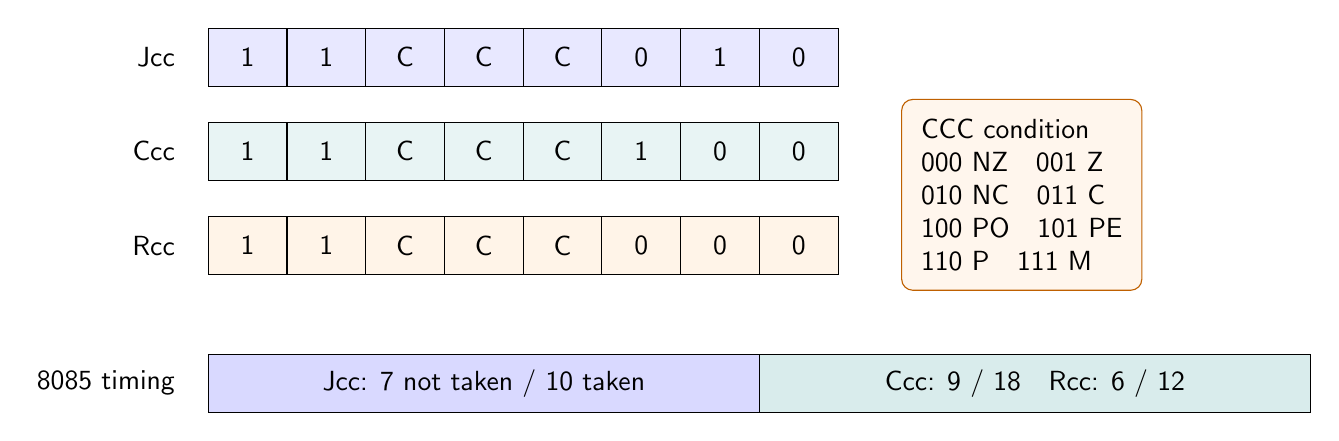
\begin{tikzpicture}[font=\sffamily,x=1cm,y=.92cm]
\node[anchor=east] at (-.3,5.4){Jcc};
\foreach \x/\v in {0/1,1/1,2/C,3/C,4/C,5/0,6/1,7/0}{\draw[fill=blue!9] (\x,5) rectangle ++(1,.8);\node at (\x+.5,5.4){\v};}
\node[anchor=east] at (-.3,4.1){Ccc};
\foreach \x/\v in {0/1,1/1,2/C,3/C,4/C,5/1,6/0,7/0}{\draw[fill=teal!9] (\x,3.7) rectangle ++(1,.8);\node at (\x+.5,4.1){\v};}
\node[anchor=east] at (-.3,2.8){Rcc};
\foreach \x/\v in {0/1,1/1,2/C,3/C,4/C,5/0,6/0,7/0}{\draw[fill=orange!9] (\x,2.4) rectangle ++(1,.8);\node at (\x+.5,2.8){\v};}
\node[draw=orange!75!black,rounded corners,fill=orange!7,align=left,anchor=west,inner sep=7pt] at (8.8,3.5) {CCC condition\\000 NZ\quad001 Z\\010 NC\quad011 C\\100 PO\quad101 PE\\110 P\quad111 M};
\node[anchor=east] at (-.3,.9){8085 timing};
\draw[fill=blue!15] (0,.5) rectangle (7,1.3);\node at (3.5,.9){Jcc: 7 not taken / 10 taken};
\draw[fill=teal!15] (7,.5) rectangle (14,1.3);\node at (10.5,.9){Ccc: 9 / 18\quad Rcc: 6 / 12};
\end{tikzpicture}
\end{document}
